\documentclass[11pt]{article}
\usepackage[margin=.73in]{geometry}
\usepackage{lmodern,amsmath,amssymb,booktabs,graphicx,microtype,fancyhdr,xurl,hyperref}
\hypersetup{colorlinks=true,urlcolor=blue,linkcolor=black}
\pagestyle{fancy}\fancyhf{}\lhead{HPS GPR: v16 signal templates and fit windows}\rhead{v6.3.7}\cfoot{\thepage}
\setlength{\headheight}{14pt}\setlength{\parindent}{0pt}\setlength{\parskip}{6pt}\setlength{\emergencystretch}{2em}
\begin{document}
\section*{Appendix D. v6.3.7: fit the signal-MC shape and test the window}

A Gaussian describes the narrow signal core, but it does not describe all selected signal events. This study asks whether using the measured core and tails improves the extraction of a known injected signal. It also asks how much mass range to fit and how much to remove from Gaussian-process (GP) background training. Better shape agreement alone does not guarantee a better upper limit: removing more sideband bins weakens the background prediction.

The inputs are verified v16 target-constrained (TC) signal Monte Carlo: stored reconstructed masses binned at 0.1 MeV, normalized to all selected candidates including overflow. The new templates use simulated masses from 80 to 240 MeV. The acceptance-turn-on sample at 60 MeV is not used to predict shapes in this interval. No extrapolation is made outside it. UC inference is not attempted because there is no matching UC background source histogram.

\textbf{Two different intervals.} Let $F$ denote the bins included in the signal likelihood, and $G$ the bins excluded from GP training. The coordinate is
\[
 u=\frac{m_{\rm rec}-c(m)}{\sigma_{\rm core}(m)}.
\]
Here $c(m)$ and $\sigma_{\rm core}(m)$ are predicted signal-core quantities. They are different from the reference analysis resolution used by the original shifted Gaussian. The proposed starting exclusion is $G_0=[-4,3]$ in $u$. To avoid using a count both to train the background and to fit the signal, this implementation requires
\[
 F\subseteq G,\qquad G=G_0\cup F\quad\hbox{when extending the starter fit.}
\]
Thus extending the fitted template by two core widths on each side changes both the fitted interval and the actual GP exclusion to $[-6,5]$. A guard-only extension, which removes training bins without fitting them, tests a different tradeoff. The GP kernel parameters remain frozen; its background mean and covariance are recomputed from each toy's remaining sidebands.

\textbf{What a fitted yield means.} The expected yield $A$ counts all selected signal events. Every injected toy uses the full signal-MC distribution, including tails in GP training bins and events outside the background spectrum. For a template probability $p_i$, the signal expectation in fitted bin $i$ is $A p_i$. If the fit retains probability $f_F$, its expected signal count is $A f_F$. We never renormalize the retained bins to unit probability. Shortening the fit therefore cannot make physical leakage disappear.

The GP mean background source generates Poisson count fluctuations about the archived mean spectrum. It does not draw a random GP function for each toy. These are conditional sensitivity studies using the selected signal production and the archived background model, not a new observed-data search. The main-body v6.3.6 observed fits and limits are unchanged.
\clearpage\section*{Appendix E. Predict an intermediate mass from its neighbors}

For a tested mass $m$ between simulated masses $m_L$ and $m_R$, set $t=(m-m_L)/(m_R-m_L)$. Interpolate the core center and width,
\[
 c_m=(1-t)c_L+t c_R,\qquad s_m=(1-t)s_L+t s_R.
\]
For each anchor, define its complete aligned cumulative distribution $C_j(u)=P_j[(m_{\rm rec}-c_j)/s_j\le u]$. The prediction is
\[
 F_m(x)=(1-t)C_L\!\left(\frac{x-c_m}{s_m}\right)
        +t C_R\!\left(\frac{x-c_m}{s_m}\right).
\]
Bin probabilities are differences of this cumulative distribution at bin edges. The weights are nonnegative and sum to one, so the construction preserves probability and moves both the core and the tails. The recorded overflow remains an unresolved upper-tail category; it is not assigned invented mass positions.
\begin{center}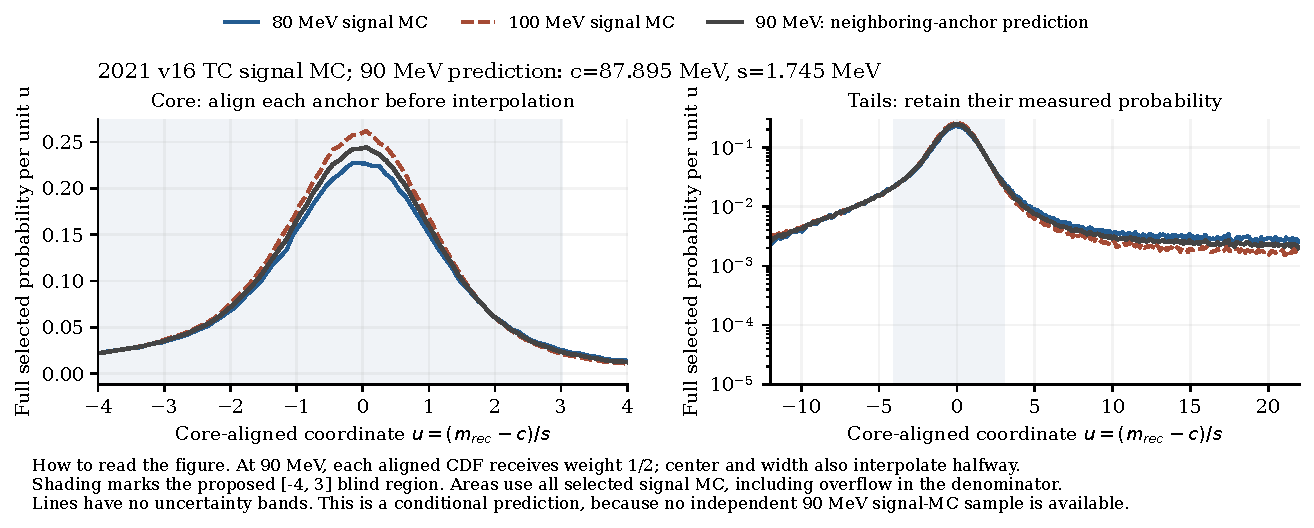
\includegraphics[width=\linewidth,height=3.65in,keepaspectratio]{../figures/v637_neighbor_interpolation.pdf}\end{center}
{\small\textbf{Figure 1.} \textbf{How to read the figure.} The 90 MeV model interpolates the 80 and 100 MeV signal-MC samples with equal weights after aligning each fitted core. Both the fitted core location and width interpolate linearly; the complete aligned CDF carries the tails. The left panel resolves the core and the right panel resolves small tail probabilities on a logarithmic scale. The shaded interval is the proposed training exclusion [-4,3]. The 90 MeV curve is a conditional prediction, not closure against an independent sample. No uncertainty bands are shown.}\par\medskip

At 90 MeV, the fitted core is predicted at 87.895 MeV with width 1.745 MeV. Both aligned signal distributions receive weight one half. This implements the requested intermediate core and tails. It is related to the alignment-and-mixing idea in template morphing [1]; the core-fit parameters used here are not the full moments of that method.

The \textbf{common-shape comparator} instead averages the full aligned distributions at all retained anchor masses with equal weight. Its target center and width still come from the nearest two masses. Comparing it with neighboring-template interpolation isolates the benefit of local tail information.
\clearpage\section*{Appendix E. Predict samples that were removed from the model}
\begin{center}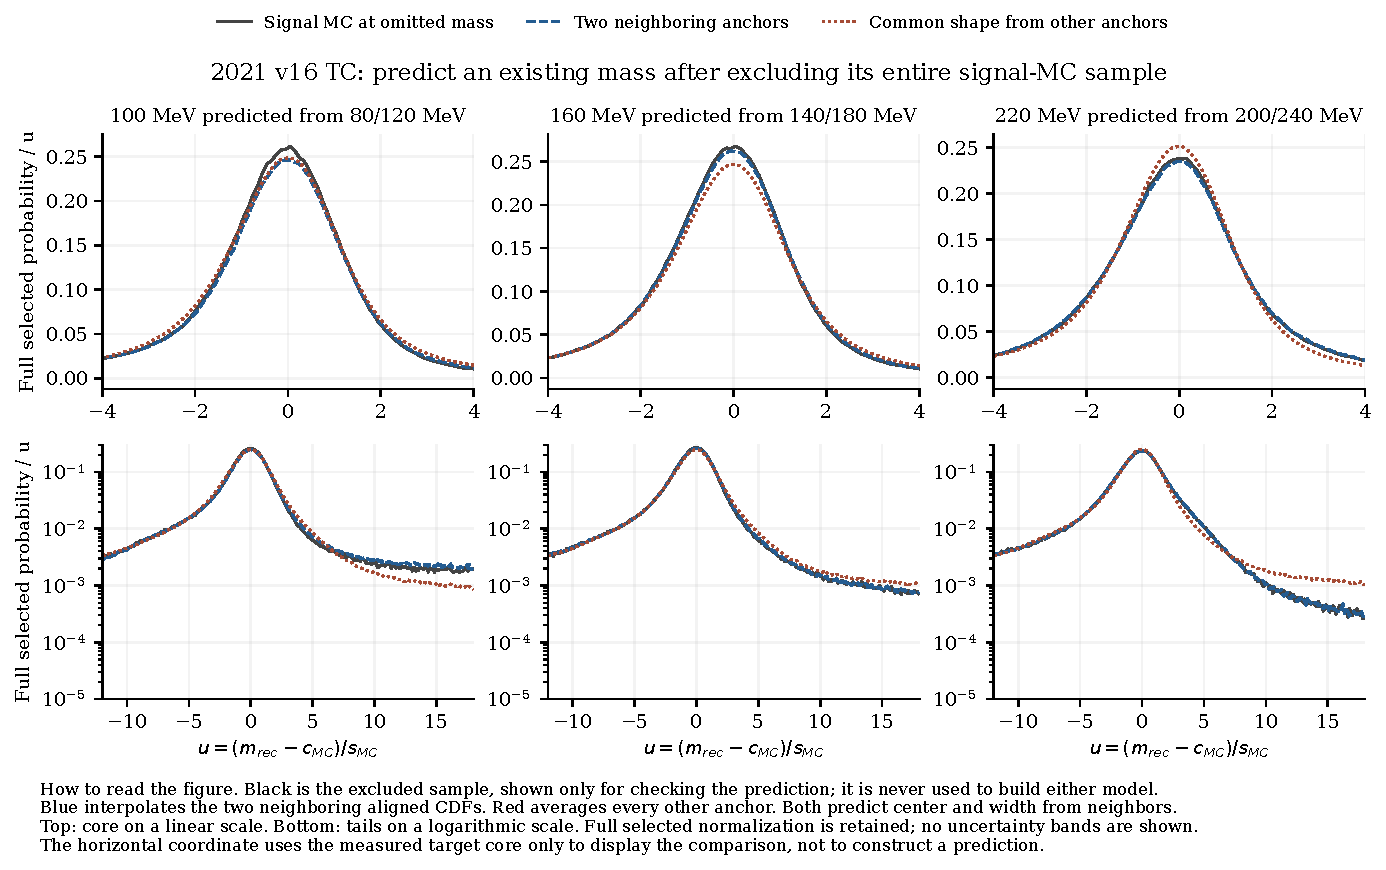
\includegraphics[width=\linewidth,height=5.0in,keepaspectratio]{../figures/v637_omitted_mass_shapes.pdf}\end{center}
{\small\textbf{Figure 2.} \textbf{How to read the figure.} At each displayed mass, the black signal-MC distribution is excluded from model construction and then used to check the prediction. Blue interpolates the two adjacent samples, including core and tails. Red uses the equal-weight common shape from all other anchors. Both models predict the target center and width from its neighbors. Upper panels show the core, and lower panels show the tails. All densities retain the full selected-event normalization; no fit-window renormalization or uncertainty bands are applied.}\par\medskip

The signal-MC sample at the tested mass is removed from both template construction and the prediction of its core parameters. It is then used as the independent shape target. For example, the 100 MeV prediction uses 80 and 120 MeV; the 160 MeV prediction uses 140 and 180 MeV. This is more demanding than reproducing an anchor, where interpolation equals the input histogram by construction.

Neighboring-template interpolation captures the mass dependence of the tails more closely than the common shape in this diagnostic. The largest residual occurs near the lower end of the tested range: the 100 MeV prediction must bridge the rapidly changing 80--120 MeV distributions. Similar-looking cores therefore do not justify assuming exact tail agreement.

These comparisons use the full selected normalization. Neither a good core fit nor a smaller shape discrepancy by itself establishes improved sensitivity; the independent toy study below tests that next.
\clearpage\section*{Appendix E. Quantify interpolation errors across the range}
\begin{center}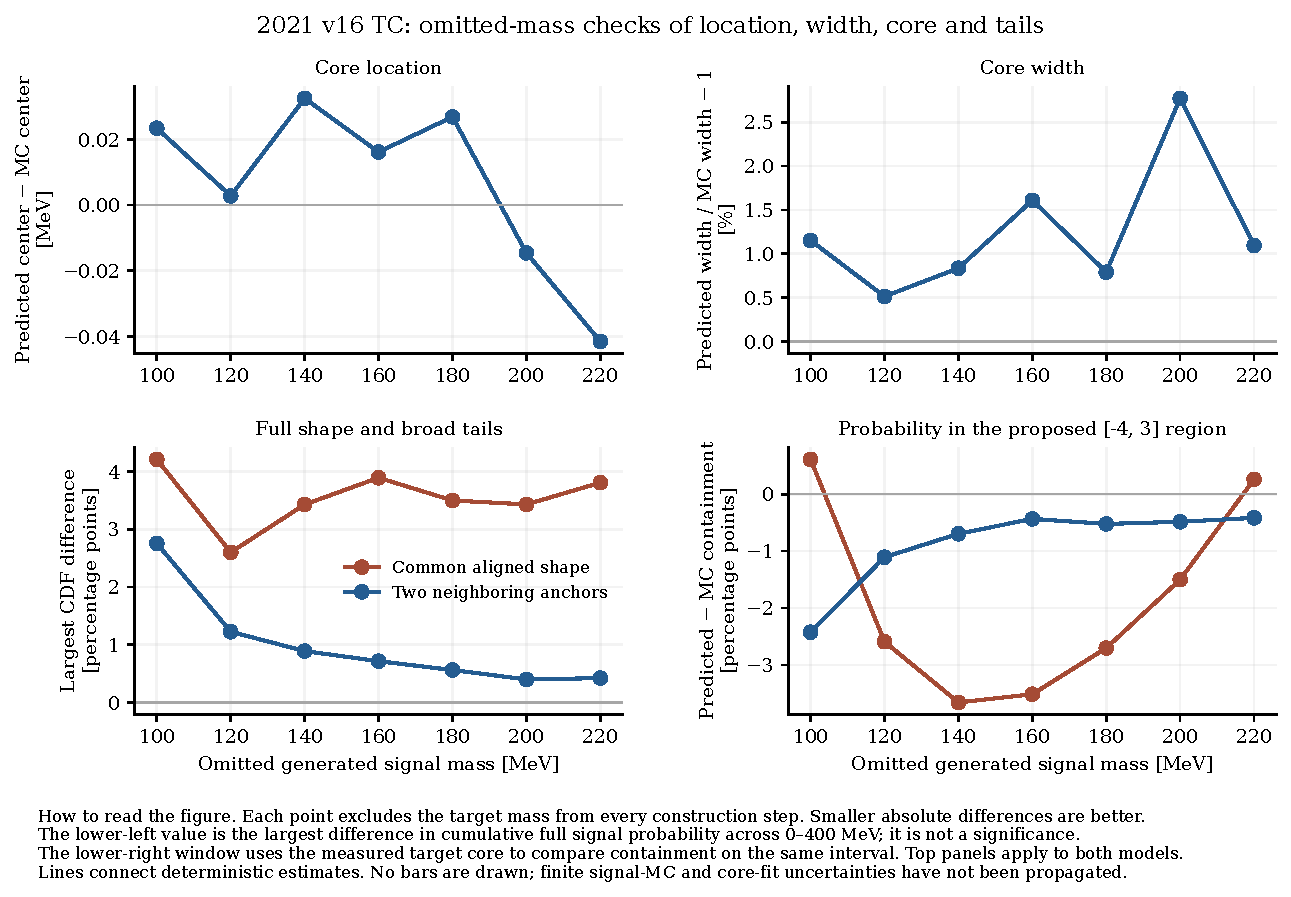
\includegraphics[width=\linewidth,height=4.5in,keepaspectratio]{../figures/v637_shape_closure_metrics.pdf}\end{center}
{\small\textbf{Figure 3.} \textbf{How to read the figure.} Each target mass is removed before predicting its center, width and distribution. The upper panels measure core-parameter errors. The lower-left panel gives the maximum absolute CDF difference, which compares integrated probability throughout the stored mass range. The lower-right panel compares probability in the same [-4,3] window defined using the excluded MC core only for evaluation. Smaller absolute differences indicate better agreement. These are deterministic shape checks; finite signal-MC and fitted-core uncertainties are not propagated, so no bars are shown.}\par\medskip

For the seven omitted masses from 100 to 220 MeV, the largest absolute cumulative-probability difference is 0.0040--0.0276 for neighboring-template interpolation, compared with 0.0260--0.0421 for the common shape. This metric asks how far the predicted integrated probability can depart from the simulated distribution at any stored mass threshold. It is not a goodness-of-fit probability or a confidence interval.

The comparison at 100 MeV has a difference of about 0.0276: an integrated probability can be wrong by about 2.8 percentage points. This remaining modeling difference is relevant even though the core looks close. Finite signal-MC statistics and the core-fit uncertainties are not propagated into the new toy calibration; the template inputs are treated as fixed.

The package checks nonnegative bin probabilities, monotone cumulative distributions, unit total probability including outside-support categories, and exact reproduction at the retained anchors. Interpolation is allowed only inside 80--240 MeV. A curve drawn at an intermediate mass is a model prediction, not new detector simulation.
\clearpage\section*{Appendix F. Choose the window before testing it}

Three simulated masses, 100, 160 and 220 MeV, span the interior of the interpolation range. Each is removed from the common and neighboring template inputs. The direct signal-MC extraction is a best-case benchmark at a known mass; it is not eligible to win an interpolation procedure that must also work between samples.

The original shifted Gaussian uses its established center and reference width, with both fit and GP exclusion at $\pm2.25\sigma_{\rm ref}$. All new windows use the center and core width predicted from neighboring samples. The Gaussian in the starter window retains its reference Gaussian width. Common, neighboring and direct MC templates in the same starter window isolate the shape comparison.
\begin{center}\small\begin{tabular}{lll}\toprule
Extraction template & Fit interval $F$ & GP exclusion $G$\\\midrule
Original shifted Gaussian & $\pm2.25\sigma_{\rm ref}$ & $\pm2.25\sigma_{\rm ref}$\\
Gaussian / common / neighbors / direct MC & $[-4,3]$ & $[-4,3]$\\
Neighbors: shortened & $[-2.5,2.25]$ & $[-2.5,2.25]$\\
Neighbors: intermediate & $[-3,2.5]$ & $[-3,2.5]$\\
Neighbors: one-unit extension & $[-5,4]$ & $[-5,4]$\\
Neighbors: two-unit extension & $[-6,5]$ & $[-6,5]$\\
Neighbors: modest unused buffer & $[-3,2.5]$ & $[-4,3]$\\
Neighbors: wide unused buffer & $[-4,3]$ & $[-6,5]$\\
\bottomrule\end{tabular}\end{center}
Except for the first row, intervals are in $u$ and the actual bin boundaries are saved in the geometry table. This gives eleven candidates. The training data and the signal-fit data are disjoint for every candidate.

\textbf{Tuning.} Use 100 GP mean-source experiments with background only and with full signal MC at $A=3s_0$. The scale $s_0$ is the archived mean Gaussian yield error from an independent 100-toy background-only pilot at that mass. The expected injected yield is the same for every candidate. Poisson signal increments and background draws are paired across methods. Measure
\[
 R=\frac{\operatorname{mean}(\widehat A_{\rm signal+background}-\widehat A_{\rm background})}{A},
 \qquad W=\frac{\operatorname{SD}(\widehat A_{\rm background})}{R}.
\]
A smaller $W$ means less fitted-yield noise after correcting the mean response to added signal. Choose one candidate for all three masses by minimizing their geometric mean $W$. This is a sensitivity proxy, not an upper limit. The choice is frozen before calibration and evaluation. The common shape with $[-4,3]$ wins; its tuning ratio to the original Gaussian is 0.9917, only a 0.8\% reduction.

\textbf{Independent test.} For each background source, generate 100 new calibration experiments and 100 separate evaluation experiments. Calibration spans $A/s_0=0,0.5,1,2,3,4,5,6,8,10,12,16$; evaluation uses $0,3,5$. The selected common shape, original Gaussian, and three other starter-window shapes are retained regardless of their ranking. The functional form background source supplies a separate stress test with its own calibration; it is not a GP-calibrated test under a mismatched source.
\clearpage\section*{Appendix F. Shorter and wider windows: the measured tradeoff}
\begin{center}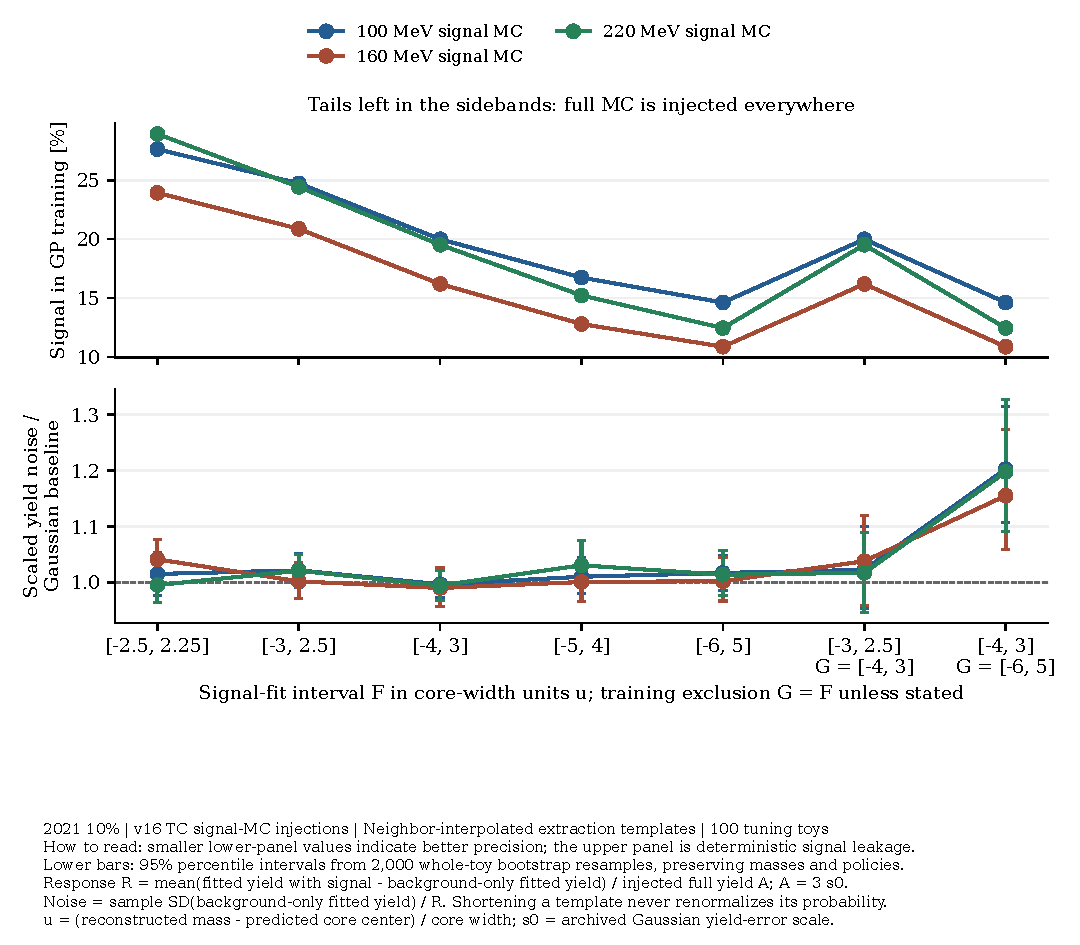
\includegraphics[width=\linewidth,height=5.0in,keepaspectratio]{../figures/v637_window_scan.pdf}\end{center}
{\small\textbf{Figure 4.} \textbf{How to read the figure.} Every curve uses full v16 TC signal-MC injections and an extraction template predicted from neighboring masses. Upper panel: fraction of all selected signal events entering GP training bins. Lower panel: background-only fitted-yield scatter divided by the signal response, relative to the original Gaussian result at that mass. Bars are 95\% percentile intervals from 2,000 whole-toy bootstrap resamples of the 100 tuning experiments, preserving mass and method correlations. $s_0$ is the archived Gaussian yield-error scale. The last two choices leave an unused buffer between fit and training. The upper panel has no uncertainty bars because the signal histogram is treated as fixed.}\par\medskip

The proposed $[-4,3]$ interval leaves 20.0\%, 16.2\% and 19.5\% of the full selected signal in GP training at 100, 160 and 220 MeV. Extending the fit and exclusion to $[-6,5]$ reduces those fractions to 14.6\%, 10.9\% and 12.4\%. They are still not negligible. All these tails are present in the simulated data.

The two-unit extension does not improve the tuning precision: its three-mass ratio is 1.0109. Excluding that wide interval while fitting only $[-4,3]$ is more costly, with ratio 1.1846. In these tests, removing background information without fitting the additional bins is worse than using the wider fit. No tested interval achieves both negligible leakage and a demonstrated sensitivity gain.
\clearpage\section*{Appendix G. Better yield response, modest sensitivity changes}
\begin{center}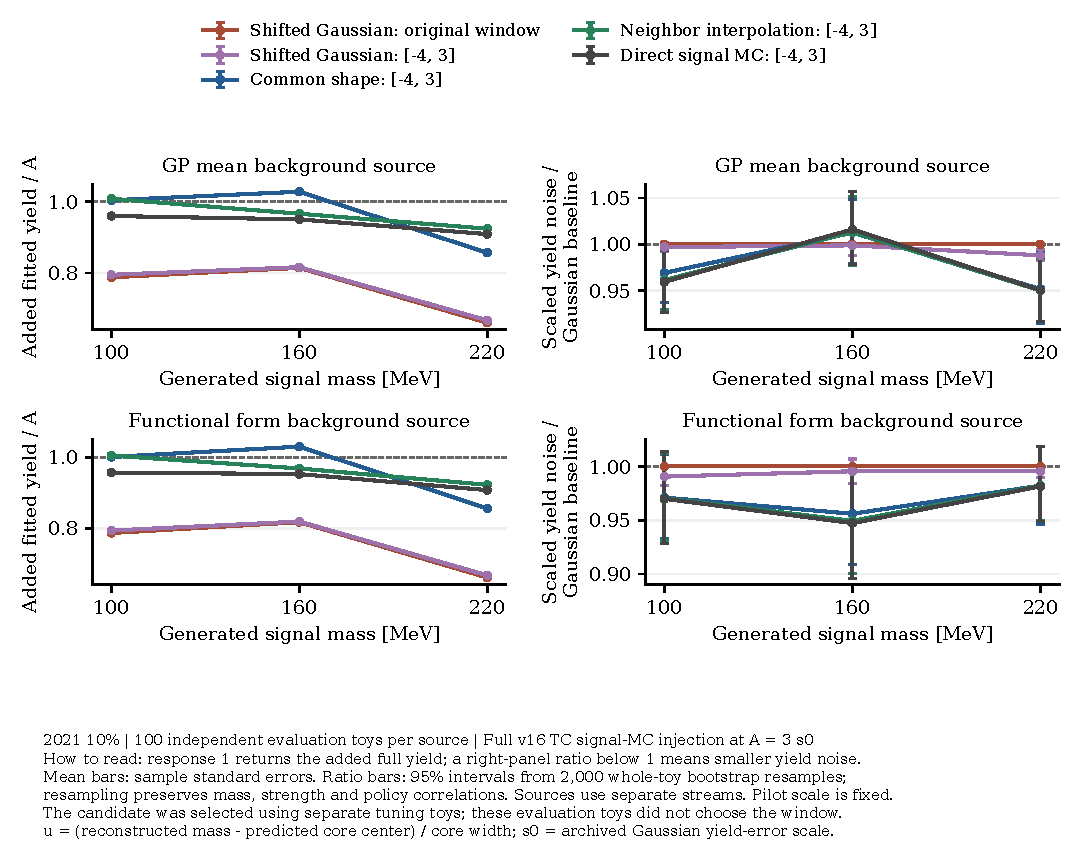
\includegraphics[width=\linewidth,height=4.2in,keepaspectratio]{../figures/v637_independent_response.pdf}\end{center}
{\small\textbf{Figure 5.} \textbf{How to read the figure.} Each point uses 100 independent evaluation experiments with expected full selected yield $A=3s_0$. Left: mean added fitted yield divided by $A$; bars are sample standard errors of the paired signal-induced change. Right: background-only yield noise divided by the response, relative to the original shifted Gaussian; bars are 95\% intervals from 2,000 whole-toy bootstrap resamples. Resampling preserves mass, strength and method correlations; sources use separate streams. The pilot scale is fixed. The common-shape window was selected on a separate tuning sample. A response closer to one does not by itself mean a smaller upper limit.}\par\medskip
\begin{center}\small\begin{tabular}{lrrr}\toprule
Mass [MeV] & Common response $R$ & Noise ratio & 95\% bootstrap interval\\\midrule
100 & 1.003 & 0.969 & [0.937, 1.000]\\
160 & 1.027 & 1.013 & [0.979, 1.048]\\
220 & 0.857 & 0.952 & [0.915, 0.992]\\
\bottomrule\end{tabular}\end{center}
For the selected common template, the geometric-mean noise ratio across the three masses is 0.9774 [0.9579, 0.9977] on the GP mean source and 0.9696 [0.9451, 0.9919] on the functional form source. These are conditional reductions of about 2--3\% in this precision diagnostic. The mass-by-mass result is mixed, including a slight increase at 160 MeV on the GP source.

The direct MC template still returns responses of about 0.959, 0.950 and 0.909 on the GP source. Even the exact signal shape in the fitted bins does not eliminate absorption of signal in the sidebands. The common shape's response can also exceed one because its mass-dependent tail fraction is imperfect. Calibration remains necessary.
\clearpage\section*{Appendix G. Toy-calibrated limits and signal detection}
\begin{center}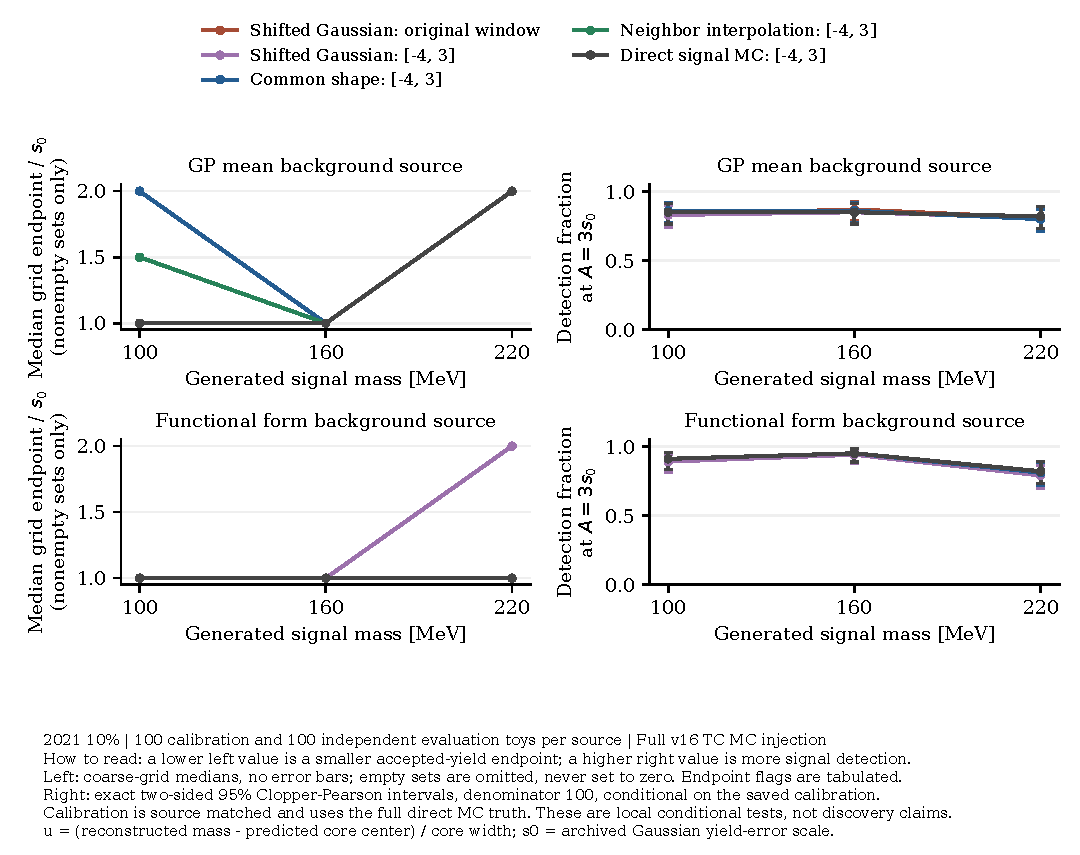
\includegraphics[width=\linewidth,height=4.15in,keepaspectratio]{../figures/v637_limits_and_detection.pdf}\end{center}
{\small\textbf{Figure 6.} \textbf{How to read the figure.} Calibration and evaluation each contain 100 experiments per source. Left: median largest accepted $A/s_0$ from the discrete yield grid, calculated among nonempty accepted sets; no error bars are assigned to these coarse medians. Empty counts are listed below. Right: fraction rejecting background only when full signal MC at $A=3s_0$ is injected. Bars are exact two-sided 95\% Clopper--Pearson intervals with denominator 100, conditional on the saved calibration sample. Calibration uses the same background source and direct signal-MC distribution as evaluation. Curves at common coordinates can overlap. These are fixed-mass local tests; a 10\% rejection threshold is not a discovery criterion.}\par\medskip
\begin{center}\small\begin{tabular}{lrrrrr}\toprule
Source & MeV & Gaussian $U/s_0$ & Empty / 100 & Common $U/s_0$ & Empty / 100\\\midrule
GP mean & 100 & 1.50 & 8 & 2.00 & 8\\
GP mean & 160 & 1.00 & 6 & 1.00 & 7\\
GP mean & 220 & 2.00 & 8 & 2.00 & 2\\
Functional & 100 & 1.00 & 11 & 1.00 & 11\\
Functional & 160 & 1.00 & 6 & 1.00 & 5\\
Functional & 220 & 2.00 & 5 & 1.00 & 5\\
\bottomrule\end{tabular}\end{center}
The endpoint comparison does not show uniformly improved upper limits. At 100 MeV on the GP source the selected common shape has a larger median endpoint, while several other comparisons tie on this coarse grid. Calibration sampling and grid spacing limit what these medians can resolve. The 2--3\% change in the precision diagnostic must not be restated as a measured 2--3\% limit improvement.
\clearpage\section*{Appendix G. What is calibrated, and what is not?}

\textbf{Upper-limit construction.} For each tested expected yield $A$, fit 100 independent calibration spectra and compare the evaluation fitted yield with that distribution:
\[
 p_A=\frac{1+\#\{\widehat A_{{\rm cal},A}\le\widehat A_{\rm eval}\}}{101}.
\]
Retain every grid value with $p_A>0.10$. The stored result is the complete accepted set. Its largest member is a grid endpoint, not an interpolated continuous upper limit. An empty set means none of the tested yields was accepted; it is never reported as a physical zero limit. A hole or acceptance of the largest tested yield would also need separate treatment.

Across all 9,000 primary evaluation fits, 205 accepted sets are empty, none has holes, and none reaches the top of the grid. The preceding table gives the relevant background-only empty counts beside each displayed endpoint median. All 100 experiments remain in rejection-rate and detection-rate denominators; only the endpoint median conditions on a nonempty set.

\textbf{Background-only test.} To test whether a fitted yield is unusually high under background only, reverse the rank comparison:
\[
 p_0=\frac{1+\#\{\widehat A_{{\rm cal},0}\ge\widehat A_{\rm eval}\}}{101}.
\]
Reject background only at $p_0\le0.10$. With exchangeable continuous calibration and evaluation statistics, this rank rule has marginal rejection probability $10/101$ under the tested hypothesis; ties make it conservative. Each realized calibration sample gives a fluctuating threshold. Binomial intervals for the evaluation counts condition on that saved threshold and do not include drawing a replacement calibration sample.

For the selected common shape, the background-only rejection counts at 100, 160 and 220 MeV are 12, 5, 9 out of 100 on the GP mean source. The corresponding functional-source counts are 4, 10, 9. These finite-sample checks are distinct from signal detection.

\textbf{Why matching the calibration truth matters.} The primary comparison calibrates every extraction method using the full direct MC distribution at the tested mass. That makes the comparison fair at those known samples, but assumes the true signal distribution is available for calibration. At an unsimulated mass, calibration must instead rely on an interpolated shape. The next page deliberately changes that assumption and checks the resulting rejection rate against the removed signal-MC sample.

\textbf{Uncertainties.} Mean bars are sample standard errors. Widths and precision ratios use 2,000 whole-toy bootstrap resamples that preserve masses, strengths and policy correlations; sources use separate streams. Binomial counts retain denominator 100 and exact two-sided 95\% Clopper--Pearson intervals. Finite signal-MC and fitted-core uncertainties remain fixed in this bounded study.
\clearpage\section*{Appendix G. Calibrate with interpolation, test against signal MC}
\begin{center}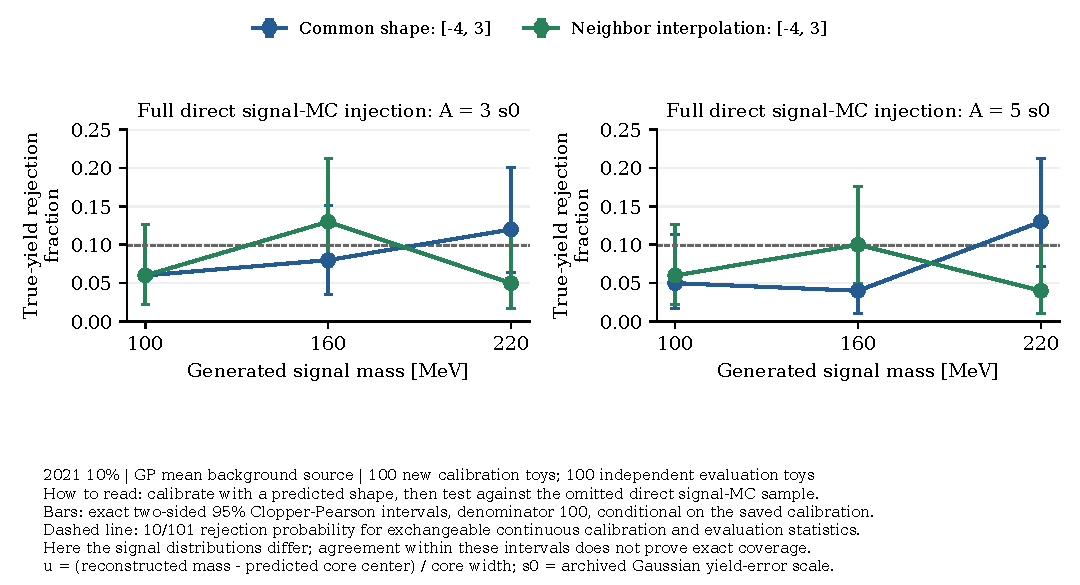
\includegraphics[width=\linewidth,height=3.6in,keepaspectratio]{../figures/v637_calibration_mismatch.pdf}\end{center}
{\small\textbf{Figure 7.} \textbf{How to read the figure.} Calibration now injects the omitted-mass common or neighboring prediction, while evaluation still injects the full direct signal-MC sample. Each method uses 100 fresh calibration experiments on the GP mean source and the same 100 independent evaluation experiments used above. Points show how often the true injected grid yield is rejected at $A=3s_0$ and $5s_0$. Bars are exact two-sided 95\% Clopper--Pearson intervals, denominator 100, conditional on that calibration sample. The dashed $10/101$ reference applies under exchangeability; shape mismatch removes that guarantee. The calibration stream differs from the primary comparison, so changes also contain finite-calibration fluctuations.}\par\medskip

At 100, 160 and 220 MeV, calibrating with the common shape rejects the true injected yield in 6, 8 and 12 of 100 experiments at $A=3s_0$, and in 5, 4 and 13 at $A=5s_0$. Neighboring-template calibration gives 6, 13 and 5 at $3s_0$, and 6, 10 and 4 at $5s_0$. Every displayed 95\% interval contains $10/101$. There are no empty sets at these two injected strengths, no holes, and no top-grid censoring.

This is a useful closure check for the practical case in which the local direct MC template is unavailable. It does not prove exact coverage or resolve small differences between the two interpolation prescriptions. Only three interior masses, two injected strengths, one background source and the fixed selected signal-MC inputs were tested in this additional diagnostic. The 90 MeV curve remains a prediction without an independent detector-MC target.

The additional study has its own frozen protocol and random-number namespace. It does not change the tuning selection or reuse the evaluation experiments to choose another window.
\clearpage\section*{Appendix H. Conclusions, sources and reproducibility}

\textbf{What v6.3.7 establishes.} The v16 neighboring-template construction predicts the full shape more accurately than a universal aligned shape in the omitted-mass checks. Both models predict the core center and width from the same neighbors. MC-informed extraction substantially improves the relation between added full signal yield and fitted yield. The selected starter-window common shape gives a modest average precision gain in independent toys, but the tested upper limits and detection fractions do not establish a uniform sensitivity improvement across masses.

\textbf{What the window study changes.} The proposed $[-4,3]$ region is a useful tested starting point, not a negligible-leakage prescription. Even the $[-6,5]$ extension leaves roughly 11--15\% of selected signal in training bins at these masses. Broadening only the exclusion while keeping a narrow fit can substantially worsen precision. The original observed-data analysis is therefore retained; the new templates and comparisons are supplied as reproducible candidates for a full mass-grid study, including selection equivalence and template uncertainty.

\textbf{Numerical record.} All 58,800 toy extraction fits passed the saved numerical checks: 6,600 tuning, 36,000 primary calibration, 9,000 independent evaluation and 7,200 interpolation-calibration fits. Thirty additional deterministic profile-limit calculations passed and are saved as asymptotic model diagnostics; they are not the toy-rank results shown here. The statistics review independently recomputed the rank tests, binomial intervals, cohort separation, pairing, geometry and normalization. No new observed-data fit or UC upper limit was made.

\textbf{Reproduce the study.} The package includes the v16 histograms, fitted core summaries, archived background spectra and kernel parameters, complete toy-fit rows, signal-category draws, random seeds, frozen candidate selection and accepted yield sets. Input hashes identify the analyzed data. The scripts \path{validate_shapes.py}, \path{run_study.py}, \path{calibration_mismatch.py}, \path{summarize_global.py}, \path{audit_statistics.py}, \path{make_figures.py} and \path{build_report.py} rebuild the numerical checks, figures and report locally. Checkpoints verify their protocol and row hashes before reuse. The updated v6.3.6 package embeds this study in \path{appendix_v637/}; previous releases are preserved separately.

\textbf{Literature and its role.}

[1] M. Baak, S. Gadatsch, R. Harrington and W. Verkerke, \emph{Interpolation between multi-dimensional histograms using a new non-linear moment morphing method}, NIM A771 (2015) 39--48, \href{https://arxiv.org/abs/1410.7388}{arXiv:1410.7388}. This motivates aligning location and width before mixing templates and testing predictions against omitted simulations. Our empirical core-aligned construction is related, but is not an exact implementation of moment morphing.

[2] M. Frate et al., \emph{Modeling Smooth Backgrounds and Generic Localized Signals with Gaussian Processes}, \href{https://arxiv.org/abs/1709.05681}{arXiv:1709.05681}. Its discussion of regularized GP likelihoods and injected-signal power motivates ensemble calibration of the background-plus-signal procedure; it does not validate the present kernel choices.

[3] G. Punzi, \emph{Sensitivity of searches for new signals and its optimization}, \href{https://arxiv.org/abs/physics/0308063}{arXiv:physics/0308063}. Search optimization should address detection and exclusion. Here independent toys evaluate those quantities after tuning; no counting-experiment approximation replaces the correlated GP calculation.

[4] G. Cowan et al., \emph{Asymptotic formulae for likelihood-based tests of new physics}, EPJ C71 (2011) 1554, \href{https://arxiv.org/abs/1007.1727}{arXiv:1007.1727}. This supplies the context for the separately saved asymptotic profile-limit diagnostics, not a coverage guarantee for these two-stage GP fits.

\end{document}
